% !TEX root = ../diploma.tex
\section{Физиология}
\subsection{Cубфизиология}

Частота пульса у взрослых кошек варьирует в зависимости от физической и психической активности и составляет от 120 до 220 ударов в минуту. Частота дыхания составляет в среднем 20—40 дыхательных движений в минуту.

\[x^n = \mathbb{R}^n + y^n\]

\section{Вопрос о полном одомашнивании}

В наше время среди учёных нет точного ответа, является ли кошка полностью одомашненным животным, так как, например, собака в процессе одомашнивания изменила свою модель поведения, сумев развить довольно сильную привязанность и преданность к человеку, и одновременно утратила множество способностей к охотничьему образу жизни и сигнальному общению, присущих её предкам — волкам.

\begin{figure}
	\centering
	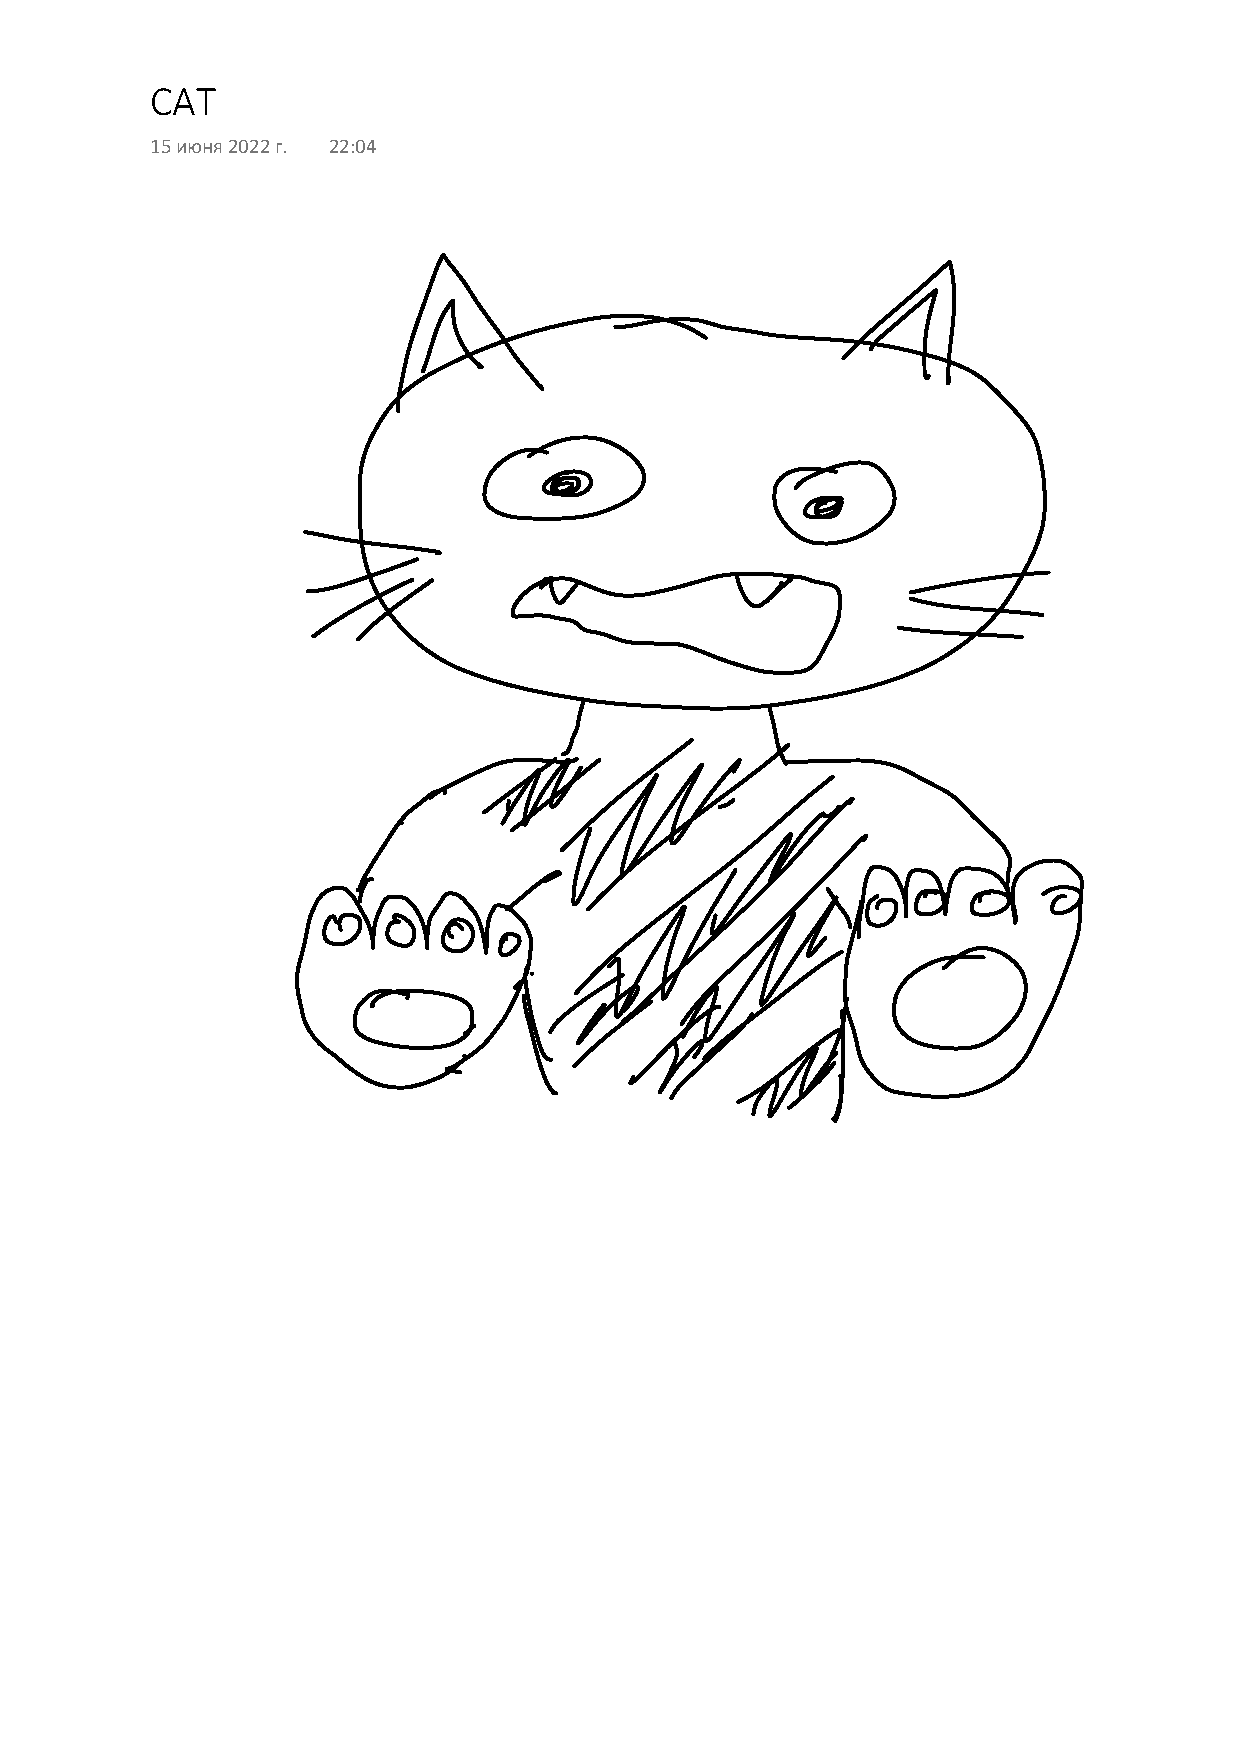
\includegraphics[clip, trim=2cm 2cm 2cm 2cm, width=0.3\textwidth]{cat}
	\caption{Название $\mathbf{Cat}$}
	\label{fig:im1}
\end{figure}

На картинке \ref{fig:im1}, смотреть в \cite{betti}.